\documentclass[11pt,a4paper]{article}

% ===== PACKAGE IMPORTS =====
% Essential packages for document formatting and functionality
\usepackage[utf8]{inputenc}
\usepackage[T1]{fontenc}
\usepackage{lmodern}
\usepackage[margin=1in]{geometry}
\usepackage{xcolor}
\usepackage{colortbl}
\usepackage{hyperref}
\usepackage{graphicx}
\usepackage{enumitem}
\usepackage{booktabs}
\usepackage{listings}
\usepackage[breakable,skins,theorems]{tcolorbox}
\usepackage{titlesec}
\usepackage{fancyhdr}
\usepackage{multirow}
\usepackage{wrapfig}
\usepackage{microtype}
\usepackage{pdfpages}  % Add this to your package imports
\usepackage{bookmark}  % Add this to your package imports
\usepackage{caption}   % Add this for \captionof command

% ===== COLOR DEFINITIONS =====
% Standard document colors
\definecolor{codebackground}{rgb}{0.95,0.95,0.95}
\definecolor{commandcolor}{rgb}{0.8,0.0,0.0}
\definecolor{outputcolor}{rgb}{0.0,0.0,0.6}
\definecolor{commentcolor}{rgb}{0.4,0.8,0.4}
\definecolor{sectioncolor}{rgb}{0.0,0.3,0.5}
\definecolor{subsectioncolor}{rgb}{0.0,0.4,0.4}
\definecolor{subsubsectioncolor}{rgb}{0.0,0.5,0.7} % New color for
% subsubsections
\definecolor{warningcolor}{rgb}{0.9,0.5,0.3}
\definecolor{tiphighlight}{rgb}{0.95,0.95,0.7}

% terminal output styling
\definecolor{kalibackground}{rgb}{0.15,0.15,0.15}
\definecolor{kalitext}{rgb}{0.4,0.7,1.0}
\definecolor{kaliprompt}{rgb}{0.2,0.8,0.8}
\definecolor{kalicommand}{rgb}{0.4,0.7,1.0}
\definecolor{kalioutput}{rgb}{0.4,0.7,1.0}
\definecolor{kaliurl}{rgb}{0.4,0.7,1.0}
\definecolor{kaliheader}{rgb}{0.4,0.7,1.0}

% ===== HYPERREF SETTINGS =====
% Configure hyperlinks appearance
\hypersetup{
  colorlinks=true,
  linkcolor=sectioncolor,
  urlcolor=blue,
  citecolor=green
}

% ===== HEADER & FOOTER SETUP =====
\pagestyle{fancy}              % Use fancy page style
\fancyhf{}                     % Clear all header/footer fields
\rhead{Cybersecurity Notes}    % Right header
\lhead{Nmap Cheatsheet}        % Left header
\rfoot{Page \thepage}          % Right footer
% \lfoot{\today}                 % Left footer with current date

% ===== SECTION TITLE FORMATTING =====
% Format section headings with custom colors
\titleformat{\section}
{\color{sectioncolor}\normalfont\Large\bfseries}
{\color{sectioncolor}\thesection}{1em}{}

\titleformat{\subsection}
{\color{subsectioncolor}\normalfont\large\bfseries}
{\color{subsectioncolor}\thesubsection}{1em}{}

% Change subsubsection numbering to Roman numerals while keeping the
% full hierarchy
\renewcommand{\thesubsubsection}{\thesubsection.\Roman{subsubsection}}

\titleformat{\subsubsection}
{\color{subsubsectioncolor}\normalfont\normalsize\bfseries}
{\color{subsubsectioncolor}\thesubsubsection}{1em}{}

% ===== CUSTOM ENVIRONMENTS =====
% Command box environment for terminal commands and output
\newenvironment{commandbox}[1][]{
  \begin{tcolorbox}[
      colback=kalibackground,
      colframe=commandcolor,
      fonttitle=\bfseries\color{white},
      title=#1,
      breakable=true
    ]
  }{
  \end{tcolorbox}
}

% Tip box environment for highlighting important information
\newenvironment{tipbox}[1][Tip]{
  \begin{tcolorbox}[
      colback=tiphighlight,
      colframe=warningcolor,
      fonttitle=\bfseries\color{white},
      title=#1
    ]
  }{
  \end{tcolorbox}
}

% ===== CODE LISTING SETTINGS =====
% Configure how code listings appear
\lstset{
  backgroundcolor=\color{kalibackground},
  basicstyle=\footnotesize\ttfamily\color{warningcolor},
  breakatwhitespace=false,
  breaklines=true,
  captionpos=b,
  commentstyle=\color{commentcolor},
  keepspaces=true,
  keywordstyle=\color{kalitext},
  showspaces=false,
  showstringspaces=false,
  showtabs=false,
  tabsize=2,
  moredelim=[il][\color{commentcolor}]{\$\ },
  stringstyle=\color{kalitext}
}

% Add a specific setting for bash listings where # should be a comment
\lstdefinestyle{bash}{
  morecomment=[l][\color{commentcolor}]{\#}
}

% ===== CUSTOM COMMANDS =====
% Command for source links with consistent styling
\newcommand{\sourcelink}[2]{\href{#2}{\textcolor{blue}{#1}}}

% Add this before \begin{document}
\setcounter{tocdepth}{3}  % This makes subsubsections appear in TOC

\begin{document}

% ===== TITLE SECTION =====
\begin{center}
  \begin{tcolorbox}[width=\textwidth, colback=sectioncolor!20,
    colframe=sectioncolor]
    \centering
    {\Huge \textbf{Nmap Cheatsheet}}\\[0.5em]
  \end{tcolorbox}
\end{center}

\tableofcontents
\clearpage

% ===== INTRODUCTION =====
\vspace{1em}
\begin{tcolorbox}[colback=codebackground, colframe=warningcolor]
  This document shall contain Quick-and-Dirty notes about
  nmap. I must keep it up-to-date because I feel a bit inundated in
  this cybersecurity journey to be frank.
\end{tcolorbox}

\section{Basic Nmap Commands}

% ===== SERVICE VERSION DETECTION SECTION =====
\subsection{Service and Version Detection (-sV)}

This is the Service Detection flag \textit{(yes; \texttt{-sV} is a
single flag, not a combination of both \texttt{s} AND \texttt{V})},
which will tell you the name and description of the identified services.
\begin{commandbox}[Service and Version Detection]
  % Command input with warningcolor (orange/rust)
\begin{lstlisting}[language=bash, style=bash, basicstyle=\small\ttfamily\color{warningcolor}]
$ sudo nmap -sV {target_IP}
\end{lstlisting}

  % Command output with kalitext color (blue)
\begin{lstlisting}[basicstyle=\small\ttfamily\color{kalitext}, language=bash]
Starting Nmap 7.80 ( https://nmap.org ) at 2025-03-28 06:27 GMT
Nmap scan report for 10.10.171.202
Host is up (0.00011s latency).
Not shown: 994 closed ports
PORT     STATE SERVICE    VERSION
7/tcp    open  echo
9/tcp    open  tcpwrapped
13/tcp   open  daytime?
17/tcp   open  qotd?
22/tcp   open  ssh        OpenSSH 9.6p1 Ubuntu 3ubuntu13.5 (Ubuntu Linux; protocol 2.0)
8008/tcp open  http       lighttpd 1.4.74

2 services unrecognized despite returning data. If you know the service/version, please submit the following fingerprints at https://nmap.org/cgi-bin/submit.cgi?new-service :
# [Detailed fingerprint data omitted for brevity]

MAC Address: 02:89:EC:B7:74:EF (Unknown)
Service Info: OS: Linux; CPE: cpe:/o:linux:linux_kernel

Service detection performed. Please report any incorrect results at https://nmap.org/submit/ .
Nmap done: 1 IP address (1 host up) scanned in 14.00 seconds
\end{lstlisting}
\end{commandbox}

\clearpage

% ===== DEFAULT SCRIPT SCAN SECTION =====
\subsection{Default Script Scan (-sC)}

I sometimes use this one instead of \texttt{-sV} because it runs
\textit{default scripts}\footnote{Default NSE Scripts,
\href{https://nmap.org/nsedoc/categories/default.html}{Nmap.org}},
which can give out additional information depending on the services
running on the target. You can see a comparison in outputs between
the two flags in the two boxes below.
\begin{commandbox}[Default Script Scan]
  % Command with comment - note that # starts a comment that will be
  % colored green
\begin{lstlisting}[language=bash, style=bash, basicstyle=\scriptsize\ttfamily\color{warningcolor}, breaklines=true, breakindent=0pt]
$ sudo nmap -p- -sC {target_IP} # Do you notice how I had to scan all ports, not just the top 1000 most common?
\end{lstlisting}

\begin{lstlisting}[basicstyle=\scriptsize\ttfamily\color{kalitext}]
Starting Nmap 7.80 ( https://nmap.org ) at 2025-03-28 09:22 GMT
Nmap scan report for 10.10.219.233
Host is up (0.00024s latency).
Not shown: 65526 closed ports
PORT    STATE SERVICE
22/tcp  open  ssh
25/tcp  open  smtp
|_smtp-commands: debra2.thm.local, PIPELINING, SIZE 10240000, VRFY, ETRN, STARTTLS, ENHANCEDSTATUSCODES, 8BITMIME, DSN, CHUNKING,
| ssl-cert: Subject: commonName=debra2.thm.local
| Not valid before: 2021-08-10T12:10:58
|_Not valid after:  2031-08-08T12:10:58
|_ssl-date: TLS randomness does not represent time
53/tcp  open  domain
| dns-nsid:
|_  bind.version: 9.18.28-1~deb12u2-Debian
80/tcp  open  http
|_http-title: Welcome to nginx on Debian!
110/tcp open  pop3
|_pop3-capabilities: PIPELINING SASL UIDL STLS AUTH-RESP-CODE RESP-CODES CAPA TOP
| ssl-cert: Subject: commonName=debra2.thm.local
| Not valid before: 2021-08-10T12:10:58
|_Not valid after:  2031-08-08T12:10:58
111/tcp open  rpcbind
| rpcinfo:
|   program version    port/proto  service
|   100000  2,3,4        111/tcp   rpcbind
|   100000  2,3,4        111/udp   rpcbind
|   100000  3,4          111/tcp6  rpcbind
|_  100000  3,4          111/udp6  rpcbind
143/tcp open  imap
|_imap-capabilities: more LOGIN-REFERRALS have IDLE post-login STARTTLS listed ENABLE capabilities LOGINDISABLEDA0001 Pre-login SASL-IR OK ID LITERAL+ IMAP4rev1
| ssl-cert: Subject: commonName=debra2.thm.local
| Not valid before: 2021-08-10T12:10:58
|_Not valid after:  2031-08-08T12:10:58
993/tcp open  imaps
|_imap-capabilities: LOGIN-REFERRALS more IDLE capabilities OK post-login ENABLE listed have Pre-login SASL-IR AUTH=PLAINA0001 ID LITERAL+ IMAP4rev1
| ssl-cert: Subject: commonName=debra2.thm.local
| Not valid before: 2021-08-10T12:10:58
|_Not valid after:  2031-08-08T12:10:58
995/tcp open  pop3s
|_pop3-capabilities: PIPELINING SASL(PLAIN) UIDL USER AUTH-RESP-CODE RESP-CODES CAPA TOP
| ssl-cert: Subject: commonName=debra2.thm.local
| Not valid before: 2021-08-10T12:10:58
|_Not valid after:  2031-08-08T12:10:58
MAC Address: 02:DD:7B:88:3D:75 (Unknown)

Nmap done: 1 IP address (1 host up) scanned in 20.77 seconds
\end{lstlisting}
\end{commandbox}

\clearpage

\begin{commandbox}[Service Version Detection for Comparison]
\begin{lstlisting}[language=bash, basicstyle=\small\ttfamily\color{warningcolor}]
$ sudo nmap -sV {target_IP}
\end{lstlisting}

\begin{lstlisting}[basicstyle=\small\ttfamily\color{kalitext}]
Starting Nmap 7.80 ( https://nmap.org ) at 2025-03-28 09:21 GMT
Nmap scan report for 10.10.219.233
Host is up (0.0062s latency).
Not shown: 991 closed ports
PORT    STATE SERVICE  VERSION
22/tcp  open  ssh      OpenSSH 9.2p1 Debian 2+deb12u3 (protocol 2.0)
25/tcp  open  smtp     Postfix smtpd
53/tcp  open  domain   ISC BIND 9.18.28-1~deb12u2 (Debian Linux)
80/tcp  open  http     nginx 1.22.1
110/tcp open  pop3     Dovecot pop3d
111/tcp open  rpcbind  2-4 (RPC #100000)
143/tcp open  imap     Dovecot imapd
993/tcp open  ssl/imap Dovecot imapd
995/tcp open  ssl/pop3 Dovecot pop3d
MAC Address: 02:DD:7B:88:3D:75 (Unknown)
Service Info: Host:  debra2.thm.local; OS: Linux; CPE: cpe:/o:linux:linux_kernel

Service detection performed. Please report any incorrect results at https://nmap.org/submit/ .
Nmap done: 1 IP address (1 host up) scanned in 13.00 seconds
\end{lstlisting}
\end{commandbox}

% \clearpage

% ===== OS DETECTION SCAN SECTION =====
\subsection{OS Detection (-O)}

Nmap sends a series of TCP and UDP packets to the remote host and
examines practically every bit in the responses.

\begin{commandbox}[OS Detection Scan]
\begin{lstlisting}[language=bash, style=bash, basicstyle=\small\ttfamily\color{warningcolor}]
$ sudo nmap -O {target_IP}
\end{lstlisting}

\begin{lstlisting}[basicstyle=\small\ttfamily\color{kalitext}, language=bash, style=bash]
Starting Nmap 7.95 ( https://nmap.org ) at 2025-03-28 18:41 +03
Nmap scan report for # {redacted}
Host is up (0.0044s latency).
Not shown: 994 closed tcp ports (reset)
PORT     STATE    SERVICE
21/tcp   filtered ftp
22/tcp   filtered ssh
23/tcp   filtered telnet
53/tcp   open     domain
80/tcp   open     http
8022/tcp filtered oa-system
MAC Address: # {redacted}
Device type: general purpose
Running: Linux 3.X|4.X|5.X
OS CPE: cpe:/o:linux:linux_kernel:3 cpe:/o:linux:linux_kernel:4 cpe:/o:linux:linux_kernel:5
OS details: Linux 3.10 - 4.11, Linux 5.10 - 5.13
Network Distance: 1 hop
\end{lstlisting}
\end{commandbox}
\clearpage

% Save current position in main document
\label{before-aggressive-scan}

% Place the phantom section before including the PDF
\clearpage  % Ensure we're on a new page
\phantomsection  % Place anchor here at the top of the page
\addcontentsline{toc}{subsection}{\numberline {1.4}Aggressive Scan (-A)}

% Just include the PDF without adding any extra content
\includepdf[pages=-]{aggressive-scan.pdf}

% ===== HOST DISCOVERY COMMANDS SECTION =====
\section{Host Discovery}

\subsection{ARP Scan (-PR)}

The ARP scan, \texttt{-PR}, is what you'd typically use if you're
already in the network that you want to scan for live systems. The
\texttt{-sn} flag here is necessary because it prevents nmap from
scanning for open ports after the ARP scan.

\begin{commandbox}[ARP Scan]
\begin{lstlisting}[language=bash, style=bash, basicstyle=\small\ttfamily\color{warningcolor}]
$ sudo nmap -sn -PR 192.168.100.7/24
\end{lstlisting}

\begin{lstlisting}[basicstyle=\small\ttfamily\color{kalitext}, language=bash, style=bash, breaklines=true, breakindent=0pt]
Starting Nmap 7.95 ( https://nmap.org ) at 2025-03-29 02:07 +03
Nmap scan report for 192.168.100.1
Host is up (0.0016s latency).
MAC Address: # This will show for all the live hosts, for all the upcoming Discovery Host scans in this document, but I'll redact them just in case.
Nmap scan report for 192.168.100.9
Host is up (0.092s latency).
Nmap scan report for 192.168.100.12
Host is up (0.054s latency).
Nmap scan report for 192.168.100.13
Host is up (0.11s latency).
Nmap scan report for 192.168.100.15
Host is up (0.082s latency).
Nmap scan report for 192.168.100.16
Host is up (0.10s latency).
Nmap scan report for 192.168.100.25
Host is up (0.053s latency).
Nmap scan report for 192.168.100.28
Host is up (0.061s latency).
Nmap scan report for 192.168.100.7
Host is up.
Nmap done: 256 IP addresses (9 hosts up) scanned in 28.27 seconds
\end{lstlisting}
\end{commandbox}

\vspace{-15pt}
\begin{center}
  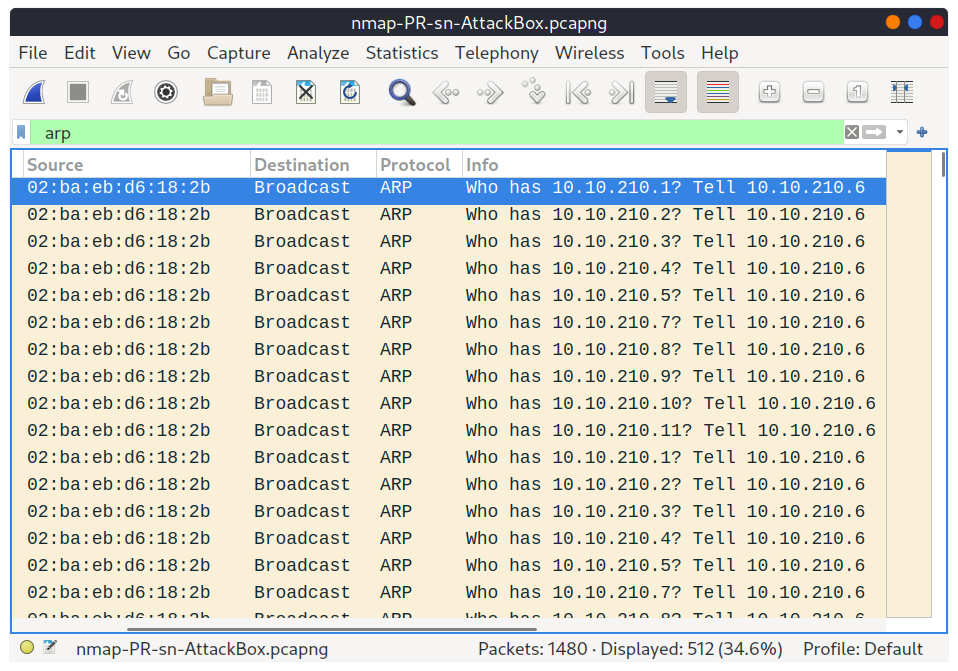
\includegraphics[width=0.7\textwidth]{arp-scan.png}
  \captionof{figure}{Wireshark capture of ARP scan packets, a network
  different from the aforementioned by the way.}
  \label{fig:arp-scan}
\end{center}

\subsection{ICMP Scans}

\begin{tcolorbox}[colback=codebackground, colframe=warningcolor]
  We'd rarely send these ICMP packets for the discovery of our
  system's own subnet, ARP Scans would be better in that case since
  firewalls tend to block ICMP packets a lot.
\end{tcolorbox}

\subsubsection{Echo Scan (-PE)}
Either way, the \texttt{-PE} scan sends the ICMP Type 8 packets (i.e.
same as your \texttt{ping} command).
\begin{commandbox}[ICMP Echo Scan (-PE)]
\begin{lstlisting}[language=bash, style=bash, basicstyle=\small\ttfamily\color{warningcolor}]
$ sudo nmap -sn -PE 192.168.100.7/24
\end{lstlisting}

\begin{lstlisting}[basicstyle=\small\ttfamily\color{kalitext}, language=bash, style=bash, breaklines=true, breakindent=0pt]
Starting Nmap 7.95 ( https://nmap.org ) at 2025-03-29 03:06 +03
Nmap scan report for 192.168.100.1
Host is up (0.0039s latency).
Nmap scan report for 192.168.100.12
Host is up (0.33s latency).
Nmap scan report for 192.168.100.13
Host is up (0.74s latency).
Nmap scan report for 192.168.100.15
Host is up (0.072s latency).
Nmap scan report for 192.168.100.16
Host is up (0.32s latency).
Nmap scan report for 192.168.100.25
Host is up (0.11s latency).
Nmap scan report for 192.168.100.28
Host is up (0.73s latency).
Nmap scan report for 192.168.100.7
Host is up.
Nmap done: 256 IP addresses (8 hosts up) scanned in 9.18 seconds
\end{lstlisting}
\end{commandbox}

\vspace{-5pt}
\noindent{\small Do you notice how it discovered 8 devices, whilst
the previous ARP scan discovered 9?}
\vspace{5pt}
\begin{center}
  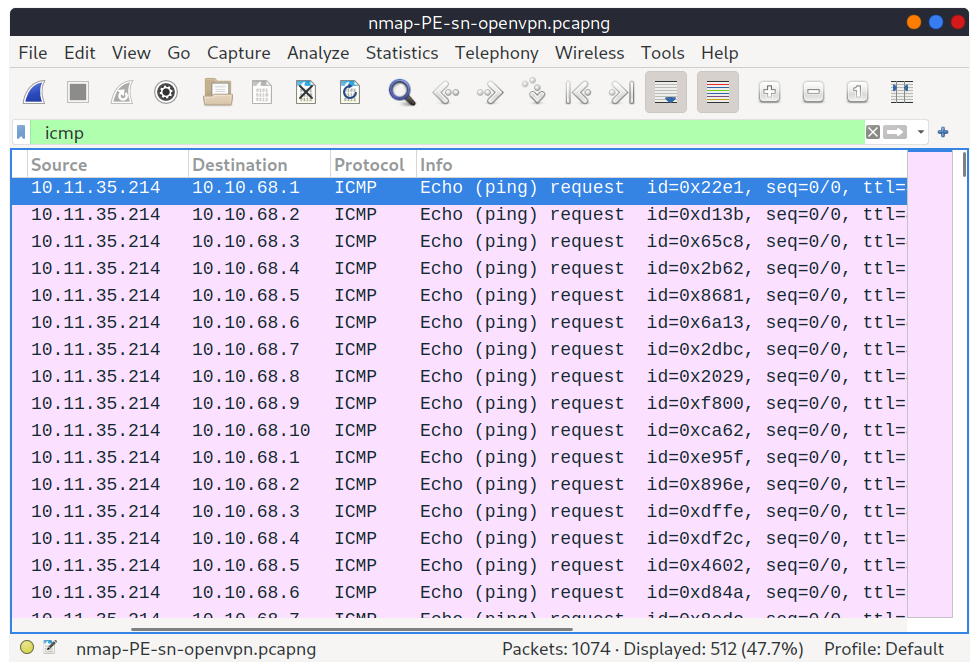
\includegraphics[width=0.7\textwidth]{echo-request.png}
  \captionof{figure}{Wireshark capture of Echo Request packets, a
  network different from the aforementioned by the way.}
  \label{fig:echo-request}
\end{center}

\clearpage

\subsubsection{Timestamp Scan (-PP)}

Because ICMP echo requests tend to be blocked, you might also
consider ICMP Timestamp (ICMP Type 13) to tell if a system is online.

\begin{commandbox}[ICMP Timestamp Scan (-PP)]
\begin{lstlisting}[language=bash, style=bash, basicstyle=\small\ttfamily\color{warningcolor}]
$ sudo nmap -sn -PP 192.168.100.7/24
\end{lstlisting}

\begin{lstlisting}[basicstyle=\small\ttfamily\color{kalitext}, language=bash, style=bash, breaklines=true, breakindent=0pt]
Starting Nmap 7.95 ( https://nmap.org ) at 2025-03-29 03:53 +03
Nmap scan report for 192.168.100.1
Host is up (0.0016s latency).
Nmap scan report for 192.168.100.9
Host is up (0.075s latency).
Nmap scan report for 192.168.100.12
Host is up (0.12s latency).
Nmap scan report for 192.168.100.13
Host is up (0.083s latency).
Nmap scan report for 192.168.100.14
Host is up (0.058s latency).
Nmap scan report for 192.168.100.15
Host is up (0.033s latency).
Nmap scan report for 192.168.100.16
Host is up (0.073s latency).
Nmap scan report for 192.168.100.25
Host is up (0.077s latency).
Nmap scan report for 192.168.100.7
Host is up.
Nmap done: 256 IP addresses (9 hosts up) scanned in 14.88 seconds
\end{lstlisting}
\end{commandbox}
\vspace{-5pt}
\noindent{\small We got "9 hosts up" once again!}

\begin{center}
  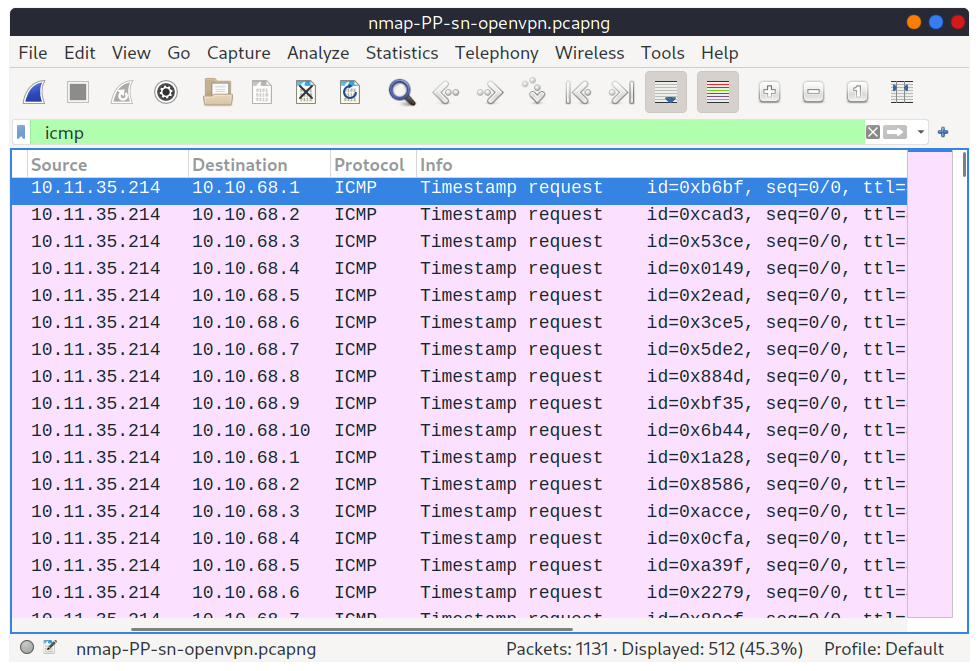
\includegraphics[width=0.7\textwidth]{timestamp-request.png}
  \captionof{figure}{Wireshark capture of Timestamp Request packets.}
  \label{fig:timestamp-request}
\end{center}

\clearpage
\subsubsection{Address Mask Scan (-PM)}

Similarly, Nmap uses address mask queries (ICMP Type 17) and checks
whether it gets an address mask reply (ICMP Type 18).

\begin{commandbox}[ICMP Address Mask Scan (-PM)]
\begin{lstlisting}[language=bash, style=bash, basicstyle=\small\ttfamily\color{warningcolor}]
$ sudo nmap -sn -PM 192.168.100.7/24
\end{lstlisting}

\begin{lstlisting}[basicstyle=\small\ttfamily\color{kalitext}, language=bash, style=bash, breaklines=true, breakindent=0pt]
Starting Nmap 7.95 ( https://nmap.org ) at 2025-03-29 03:53 +03
Nmap scan report for 192.168.100.1
Host is up (0.042s latency).
Nmap scan report for 192.168.100.12
Host is up (0.21s latency).
Nmap scan report for 192.168.100.13
Host is up (0.21s latency).
Nmap scan report for 192.168.100.15
Host is up (0.10s latency).
Nmap scan report for 192.168.100.16
Host is up (0.19s latency).
Nmap scan report for 192.168.100.25
Host is up (0.071s latency).
Nmap scan report for 192.168.100.28
Host is up (1.5s latency).
Nmap scan report for 192.168.100.7
Host is up.
Nmap done: 256 IP addresses (8 hosts up) scanned in 9.39 seconds
\end{lstlisting}
\end{commandbox}
\begin{center}
  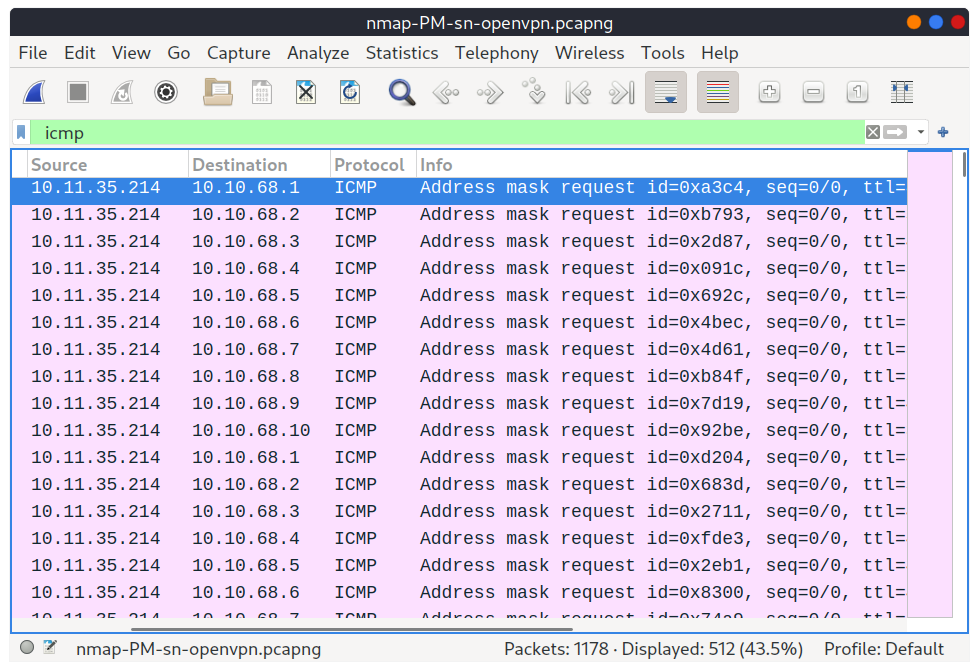
\includegraphics[width=0.7\textwidth]{addressmask-request.png}
  \captionof{figure}{Wireshark capture of Address Mask Request packets.}
  \label{fig:addressmask-request}
\end{center}

\vspace{1em}
\begin{tcolorbox}[colback=codebackground, colframe=warningcolor]
  Bonus: if you were to NOT specify one of the techniques above, just
  used \texttt{\textit{\textbf{nmap -sn}}} with no other flags,
  Nmap's default behaviour would be to reverse-DNS online hosts. And
  to skip that, you can use \texttt{\textit{\textbf{-n}}} flag.
\end{tcolorbox}
\clearpage

% Save current position in main document
\label{before-tcp-udp-discovery}

% Place the phantom section before including the PDF
\clearpage  % Ensure we're on a new page
\phantomsection  % Place anchor here at the top of the page
\addcontentsline{toc}{subsection}{\numberline {2.3}TCP/UDP Host Discovery}

% Add these lines to include the subsubsections in the TOC
\addcontentsline{toc}{subsubsection}{\numberline {2.3.I}TCP SYN Scan (-PS)}
\addcontentsline{toc}{subsubsection}{\numberline {2.3.II}TCP ACK Scan (-PA)}
\addcontentsline{toc}{subsubsection}{\numberline {2.3.III}UDP Scan (-PU)}
% Just include the PDF without adding any extra content
\includepdf[pages=-, fitpaper]{tcp-udp-discovery.pdf}

% Save current position in main document
\label{before-basic-port-scanning}

% Place the phantom section before including the PDF
\clearpage  % Ensure we're on a new page
\phantomsection  % Place anchor here at the top of the page
\addcontentsline{toc}{section}{\numberline {3}Basic Port Scanning}

% Add these lines to include the subsections in the TOC
\addcontentsline{toc}{subsection}{\numberline {3.1}TCP Connect (-sT)}
\addcontentsline{toc}{subsection}{\numberline {3.2}Stealth Scan (-sS)}
\addcontentsline{toc}{subsection}{\numberline {3.3}UDP Scan (-sU)}

% Just include the PDF without adding any extra content
\includepdf[pages=-, fitpaper]{basic-port-scanning.pdf}

% Place the phantom section before adding the content
\clearpage  % Ensure we're on a new page
\phantomsection  % Place anchor here at the top of the page

% Set the section counter to 3 so the next section will be 4
\setcounter{section}{3}
\section{Advanced Port Scanning}
\begin{tcolorbox}[colback=codebackground, colframe=warningcolor]
  Now we'll need to revise the TCP header as these scans revolve
  around manipulating its flags.
\end{tcolorbox}
\begin{center}
  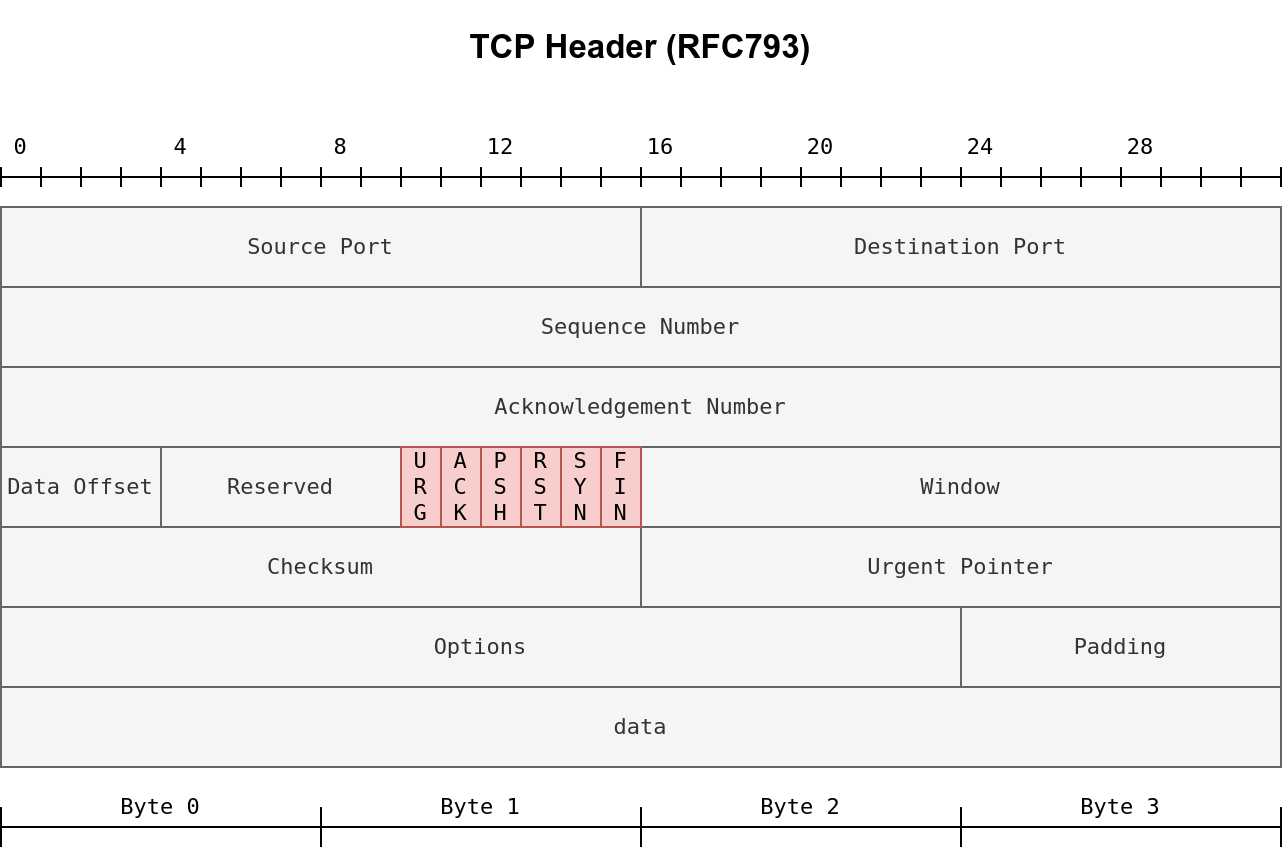
\includegraphics[width=0.7\textwidth]{./TCP-Packet}
  \label{fig:tcp-header}
\end{center}
\vspace{-5pt}
\noindent{\small Do you notice the flags in the fourth row? read em'
vertically from top to bottom if you're a little confused.}
\subsection{Null Scan (-sN)}
The null scan does not set any flag; all six flag bits are set to zero.

\begin{center}
  \includegraphics[width=0.7\textwidth]{null-open.png}
  \captionof{figure}{From Nmap’s perspective, a lack of reply in a
    null scan indicates that either the port is open or a firewall is
  blocking the packet.}
  \label{fig:null-open}
\end{center}

\begin{center}
  \includegraphics[width=0.7\textwidth]{null-closed.png}
  \captionof{figure}{We expect the target server to respond with an
  RST packet if the port is closed.}
  \label{fig:null-closed}
\end{center}

\clearpage
\subsection{FIN Scan (-sF)}
The FIN scan sends a TCP packet with the FIN flag set.

\begin{center}
  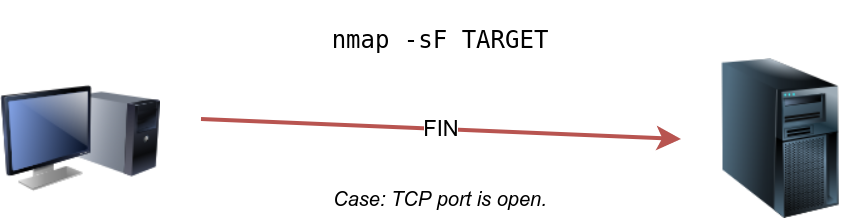
\includegraphics[width=0.7\textwidth]{FIN-Open.png}
  \captionof{figure}{Similarly, no response will be sent if the TCP
    port is open. Again, Nmap cannot be sure if the port is open or if
  a firewall is blocking the traffic related to this TCP port.}
  \label{fig:FIN-Open}
\end{center}

\begin{center}
  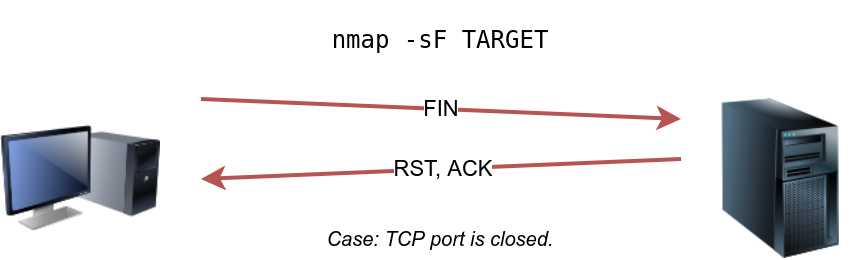
\includegraphics[width=0.7\textwidth]{FIN-Closed.png}
  \captionof{figure}{However, the target system should respond with
    an RST if the port is closed. Consequently, we will be able to know
    which ports are closed and use this knowledge to infer the ports
    that are open or filtered. It's worth noting some firewalls will
  'silently' drop the traffic without sending an RST.}
  \label{fig:FIN-Closed}
\end{center}

\subsection{Xmas Scan (-sX)}
The Xmas scan gets its name after Christmas tree lights. An Xmas scan
sets the FIN, PSH, and URG flags simultaneously. Like the Null scan
and FIN scan, if an RST packet is received, it means that the port is
closed. Otherwise, it will be reported as open|filtered. The
following two figures show the case when the TCP port is open and the
case when the TCP port is closed.

\begin{center}
  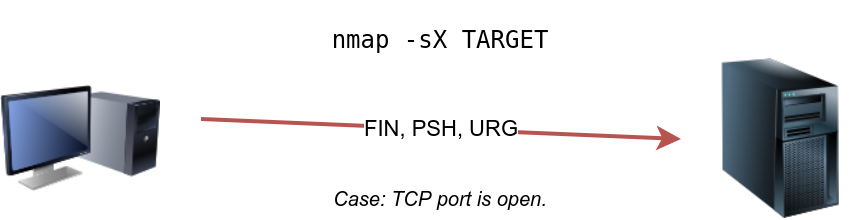
\includegraphics[width=0.7\textwidth]{Xmas-Open.png}
  \label{fig:Xmas-Open}
\end{center}

\begin{center}
  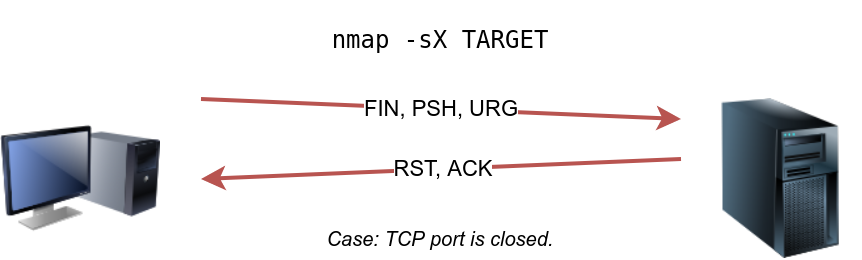
\includegraphics[width=0.7\textwidth]{Xmas-Closed.png}
  \label{fig:Xmas-Closed}
\end{center}

\clearpage

\subsection{Ack Scan (-sA)}
the target would respond to the ACK with RST regardless of the state
of the port. This behaviour happens because a TCP packet with the ACK
flag set should be sent only in response to a received TCP packet to
acknowledge the receipt of some data, unlike our case.

\begin{center}
  \includegraphics[width=0.7\textwidth]{Ack-Scan.png}
  \captionof{figure}{This kind of scan would be helpful if there is a
    firewall in front of the target. Consequently, based on which ACK
    packets resulted in responses, you will learn which ports were not
    blocked by the firewall. In other words, this type of scan is more
  suitable to discover firewall rule sets and configuration.}
  \label{fig:Ack-Scan}
\end{center}

\subsection{Window Scan (-sW)}
Another similar scan is the TCP window scan. The TCP window scan is
almost the same as the ACK scan; however, it examines the TCP Window
field of the RST packets returned. On specific systems, this can
reveal that the port is open.

\begin{center}
  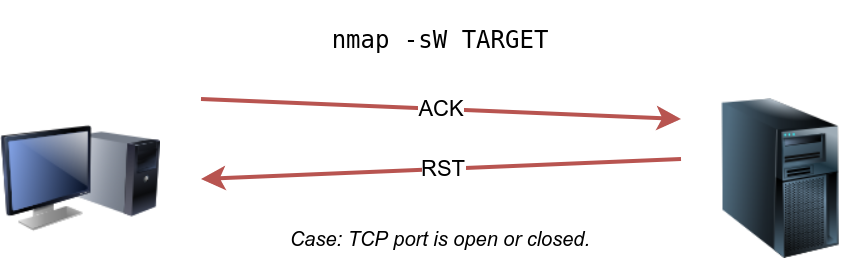
\includegraphics[width=0.7\textwidth]{Window-Scan.png}
  \captionof{figure}{This is also useful only when there's a firewall
  on the target system.}
  \label{fig:Ack-Scan}
\end{center}
\section{To Do Items}

\begin{tcolorbox}[colback=sectioncolor!20, colframe=sectioncolor,
  width=\textwidth]
  \begin{center}
    \Large\textbf{TO DO LIST}
  \end{center}

  \begin{itemize}
    \item[\textcolor{warningcolor}{$\bullet$}] \textbf{Fragmented Packets:}
      document how to attempt IDS and Firewall evansion with Nmap by fragmenting our packets using
      the \texttt{-f} option
      and other packet fragmentation techniques

    \item[\textcolor{warningcolor}{$\bullet$}] \textbf{Zombie Scan:}
      Document the \texttt{-sI} scan technique to leverage Idle Machines on the target network
      
  \end{itemize}
\end{tcolorbox}
\end{document}
